% !TEX root = main.tex

\section{Ethereum Trading Graph Analysis}
Based on effective graph analytics, we can investigate more information hidden behind transaction data on blockchain. For example, by analyzing the Ethereum trading graph (ETG, for short), accounts can be classified as different identities. 

In this section, we illustrate the construction of ETG and analyze some features which make it different from other networks or graphs.


 %we first introduce the definition of the basic concepts in trading graph embedding, and then construct multi-layer trading graph.

\subsection{Problem Definition and Modeling}
Generally, we consider the ETG as a directed graph $G=(V,E)$, where node $v \in V$ represents an account and $e \in E$ depicts the edge between two nodes. Actually, $V$ is the set of all addresses in Ethereum including both EOAs and SCs, and we use the terms address, account and node interchangeably in the remainder of this paper. $E$ is a set of ordered pairs, where $E=\{(v_i,v_j)|v_i,v_j \in V\}$. The order of an edge indicates the direction of activity (e.g., assets transfer and smart contract invocation) from $v_i$ to $v_j$.
%In our definition, each edge associates with a weight $w$, which will be discussed later. Hence, $G$ is a weighted directed graph.

The problem can be defined as follows: given ETG $G=(V,E)$, we aim to represent each node $v$ in a low-dimensional vector space $\vec{y_v}$. By representing ETG as a set of low dimensional vectors, graph analysis algorithms can then be computed efficiently. 

Typical network embedding techniques such as random-walk based and deep learning based models use the pure network structure to map into the embedding space~\cite{goyal2018capturing}. Our model is primarily motivated as an extension of GCNs (Graph Convolutional Networks), which puts the features of nodes and edges into the representation, since it shows effectiveness for entity classification in large-scale relational data~\cite{kipf2016semi}. Generally, a multi-layer Graph Convolutional Network works with the following layer-wise propagation rule:

\begin{equation}
H^{(l+1)}=\delta(\tilde{D}^{-\frac{1}{2}}\tilde{A}\tilde{D}^{-\frac{1}{2}}H^{(l)}W^{(l)})
\label{eq1}
\end{equation}

where $H^{(l)}$ is the matrix of activations in the $l$-th layer, and $W^{(l)}$ is a trainable weight matrix in the $l$-th layer. $\delta(\cdot)$ denotes an activation function such as the ReLU$(\cdot)$ = max$(0,\cdot)$. $\tilde{A}=A+I_N$ where $A$ is the adjacency matrix of the graph $G$ and $I_N$ is the identity matrix. $\tilde{D}$ is a diagonal matrix where $\tilde{D}_{ii}=\sum_{j}\tilde{A}_{ij}$.

 The method can be understood as special cases of a simple differentiable message-passing framework.

\begin{equation}
h_i^{(l+1)}=\delta(\sum_{j \in N} \frac{1}{c_{i,j}}W^{(l)}h_j^{(l)})
\label{eq:gcn}
\end{equation}

where $h_i^{(l)}$ is the hidden state of node $v_i$ in the $l$-th layer of the neural network. And $c_{ij}$ is a problem-specific normalization constant which can defined in advance such as $c_{i,j}=\sqrt{d_i d_j}$ where $d_i$ is the degree of node $v_i$.

The approach outperforms other methods such as deepwalk~\cite{perozzi2014deepwalk} in experiments on citation networks and knowledge graph dataset. However, we found that using such GCN model directly achieves poor effect on ETG which has many properties different from traditional networks (such as social media networks and citation graph). It brings the following challenges.

\begin{itemize}
\item In the original ETG, there are different relations such as assets transfer and smart contract invocation. Those relations are radically different from one another and can not be measured in a uniform weighted graph.
\item Even considering only one relationship, there are multiple edges between two nodes. For instance, repeated transactions between the same account pairs often happen. A simple method is to merge them and this will lose some information.
\item Asymmetric
%In ETG, two nodes are more similar if they have similar connection structures instead of they are just connected by an edge with larger weight simply or have similar neighborhoods. Using node adjacency as the input, most graph embedding techniques can not preserve such higher order proximity.
\end{itemize}

\subsection{Multi-relations}
\label{sec:multi-relations}
\begin{figure}[htbp]
	\centering
	\label{fig_graph_split}
	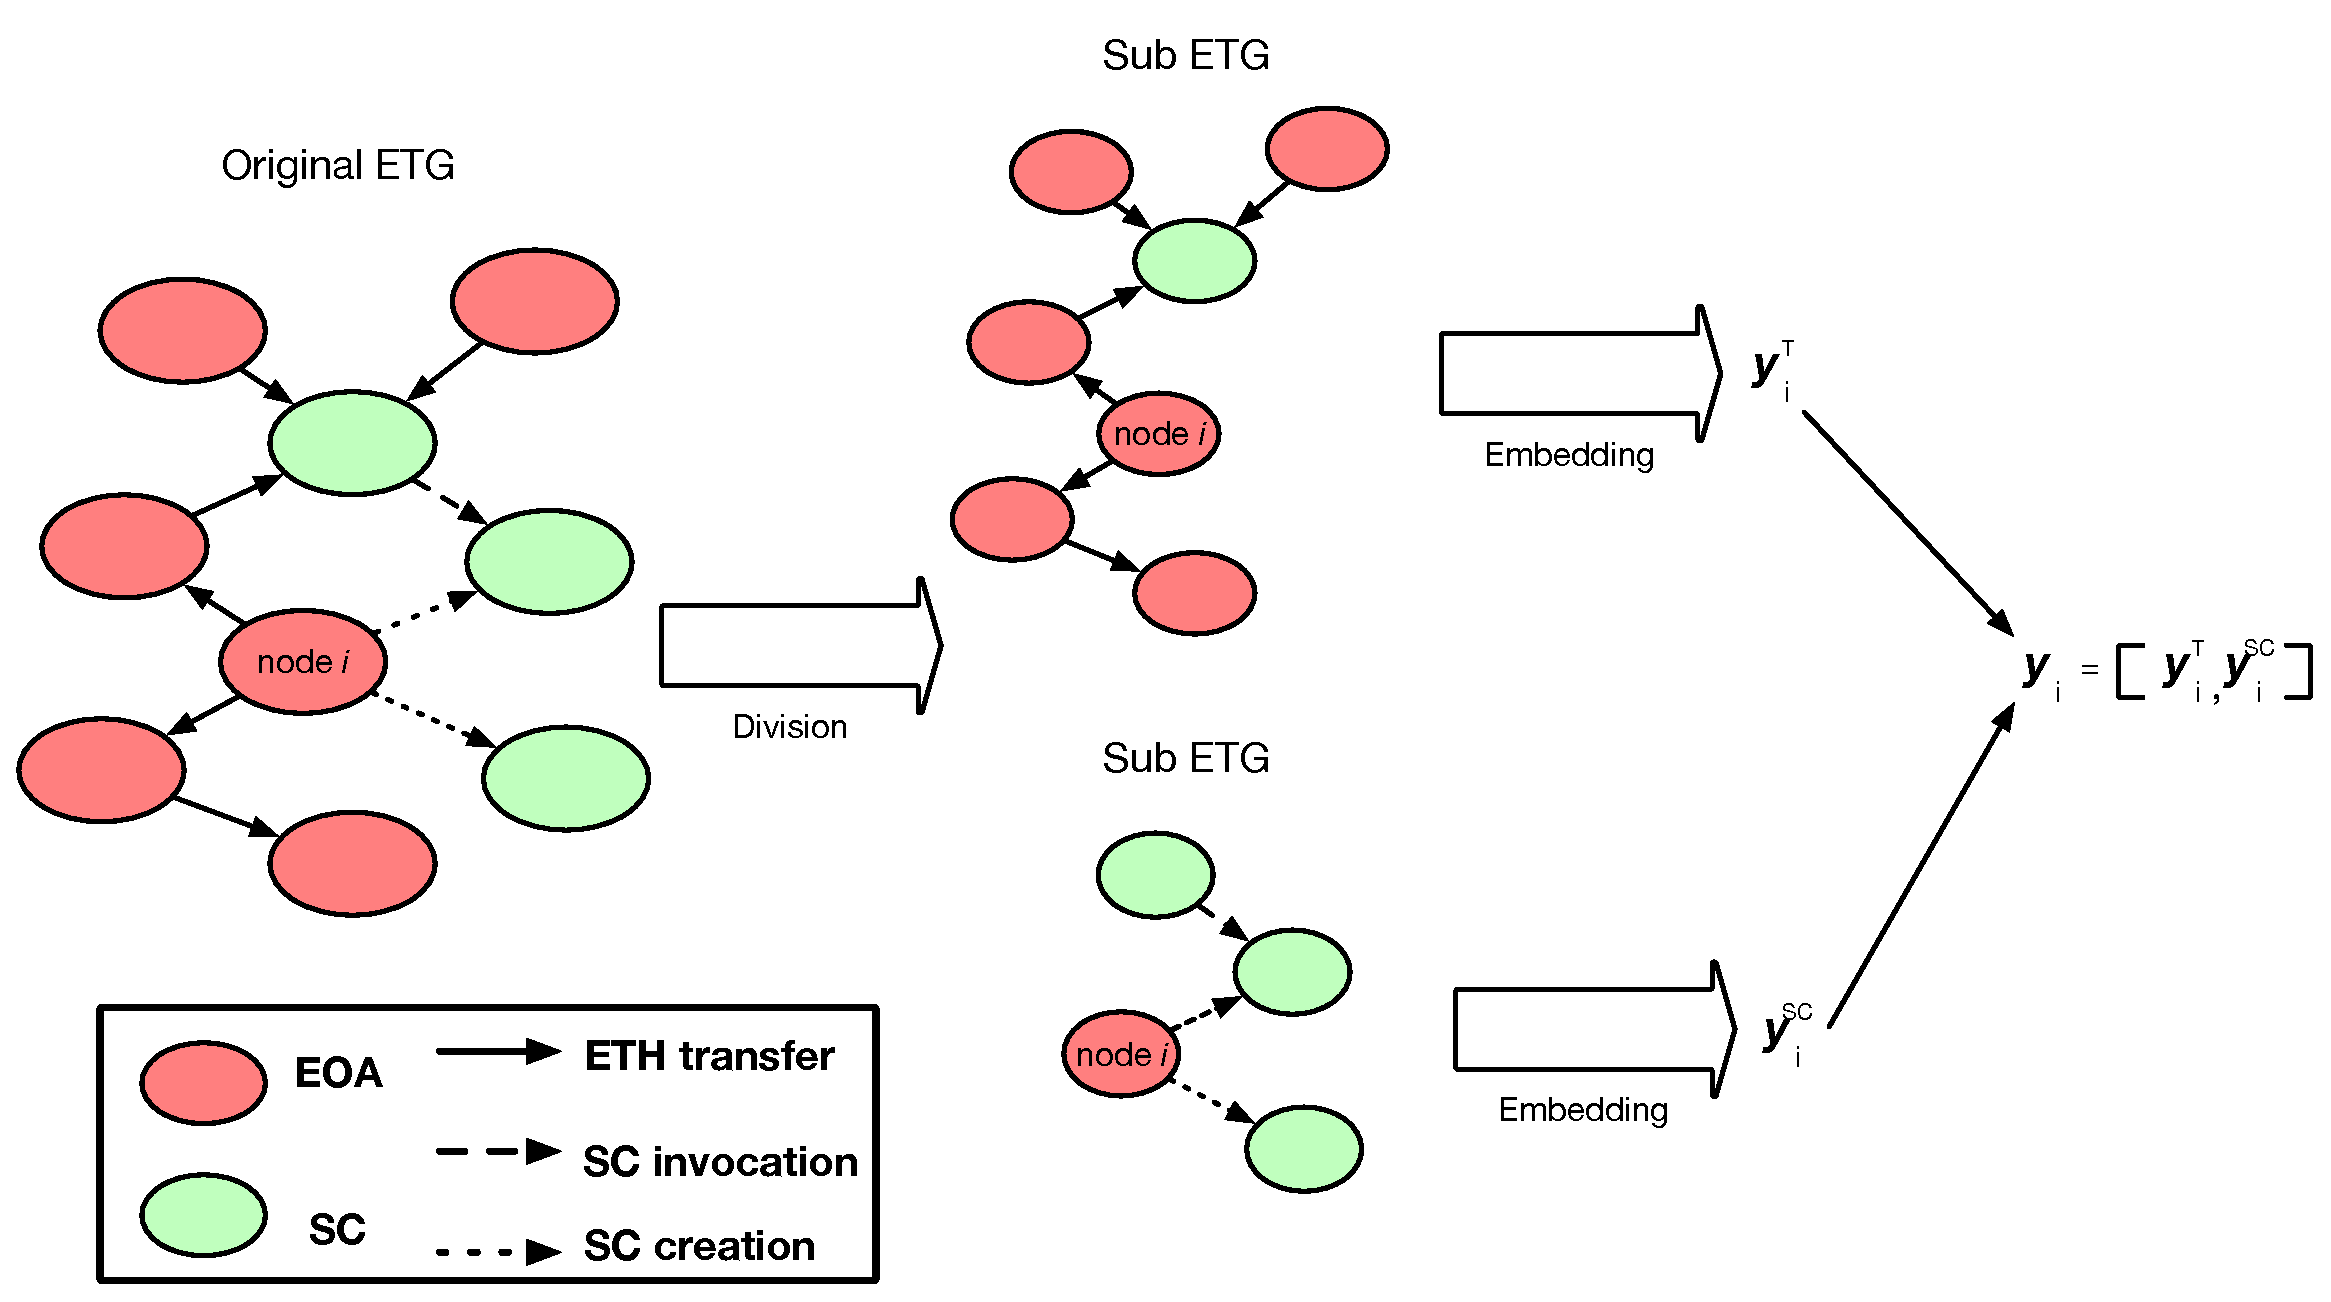
\includegraphics[width=3.5in]{fig/graph_split.eps}
	\caption{Example of a figure caption.}


	%\caption{Example of a figure caption.}
	%\label{fig_graph_split}
\end{figure}

In ETG, edges stand for different activities such as money transfer, contract creation and contract invocation, which can not be measured in a uniform weight model. For example, a weight of assets transfer maybe the ETH amount, however an invocation to smart contract does not have such numerical value. This inspired us to divide the raw ETG into different relation graphs.

%\textbf{Definition 1.} $G^{T}=\{V^T,E^T\}$, where $V^T$ is the subset of $V$. $E^T=\{(v_i,v_j,w)|v_i,v_j \in V^T,w \in \mathbb{R^+}\}$ where an edge $(v_i,v_j)$ indicates that there is at least one ETH transfer from node $v_i$ to $v_j$. And $w$ is the summation of all transferred ETH amount from $v_i$ to $v_j$ for a period of time.

%Actually, $G^T$ represents the ETH trading activities in Ethereum, and each node in $V^T$ has at least one ETH transaction.

%\textbf{Definition 2.} $G^{SC}=\{V^{SC},E^{SC}\}$, where $V^{SC}$ is the subset of $V$. $E^{SC}=\{(v_i,v_j,w)|v_i,v_j \in V^{SC},w \in \mathbb{R^+}\}$ where an edge $(v_i,v_j)$ indicates that there is at least one smart contract creation or invocation from node $v_i$ to $v_j$. And $w$ is the summation of \emph{CREATE} transaction and \emph{CALL} with $0$ ETH transactions for a period of time. 


%And $w$ is the summation of all transferred ETH amount from $v_i$ to $v_j$ for a period of time.

Relational Graph Convolutional Networks (rGCNs) is proposed to develop an encoder model for edges in the relational graph~\cite{schlichtkrull2018modeling}. The propagation model can be expressed as

\begin{equation}
h_i^{(l+1)}=\delta(\sum_{r\in R} \sum_{j \in N_i^r} \frac{1}{c_{i,r}}W_r^{(l)}h_j^{(l)}+W_0^{(l)}h_i^{(l)})
\label{eq:rgcn}
\end{equation}

where $r \in R$ represents a kind of relation ,$N_i^r$ denotes the set of neighbor indices of node $v_i$ under relation $r$, and $c_{i,r}=\frac{1}{|N_i^r|}$. Besides, single self-connection is introduced as a special relation type to each node. %compared with Eq.\ref{eq:gcn}

We divide the edge set into four relations, CALLs with ETH, CALLs without ETH, CREATIONs and REWARDs, according to the their transaction type. Note that the ERC-20 token transfers are categorized as CALLs without ETH which includes normal smart contract invocations as well. The reason is that even though ERC-20 token transfer is a kind of assets transfer intrinsically, it exists in the form of a smart contract in ETG.\footnote{Another reason is that even converting some ERC-20 tokens into ETH is available, the exchange-rate fluctuations make the unification meaningless.} % The reason is that ERC-20 token transfer is a kind of contract invocation and the transaction value is $0$ in an ERC-20 \emph{CALL} transaction.


\subsection{Time-density}
\label{section:time}
Even in a specific relation graph, there are repeated edges between the same node pairs. This occurs quite naturally since an account may transfer or invoke to another account repeatedly.

Note that these activities are located at different time intervals along the time axis which are characterized by the block height. Intuitively, a simple solution is to merge those edges by weight summation but this will lose time information. 

Here we introduce an index\textcolor{red}{?} named time-density which can be represented as strictly increasing function of block height variance.

\begin{equation}
\tau_{ij}^r=g(var(\texttt{bn}_{ij}^r))
\label{eq:time}
\end{equation}

where $\texttt{bn}_{ij}^{r}$ is the block height set of relation $r$ between node $v_i$ and $v_j$. And the new adjacency matrix in relation $r$ can be represented as 

\begin{equation}
\hat{A}=\hat{D}^{-\frac{1}{2}}(\tilde{A}+V)\hat{D}^{-\frac{1}{2}}
\label{eq:?}
\end{equation}

where $V_{ij}=\tau_{ij}$, and $\hat{D}$ is a diagonal matrix where $\hat{D}_{ii}=\sum_{j}(\tilde{A}_{ij}+V_{ij})$.

\textcolor{red}{TBA}

\subsection{High Order and Asymmetric Proximity}
In weighted graph, the edge weight $A_{ij}$ in adjacency matrix $A$ is generally treated as a measure of similarity between nodes $v_i$ and $v_j$. And the higher the edge weight, the more similar the two nodes are expected to be. Edges weight $A_{ij}$ is called \emph{first-order proximity} between nodes $v_i$ and $v_j$. 

Further, \emph{second-order} compares the neighborhood of two nodes and treat them as similar if they have a similar neighborhood~\cite{goyal2018graph}. 

However, in ETG, two nodes are more similar if they have similar connectivity structures instead of they are just connected by an edge with larger weight or share similar neighborhoods. As shown in Figure \ref{fig:high_order}, nodes $v_a$ and $v_c$ are smart contracts and node $v_b$ is normal user. Obviously, $v_a$ is not adjacent to $v_c$  but they have similar neighbor structure. Embedding models with \emph{first-order proximity} and \emph{second-order proximity} will keep them far apart although they have similar connection structures. 

\begin{figure}[htbp]
	\centering
	\subfigure[Example of a high-order proximity caption.]{
		\label{fig:high_order}
		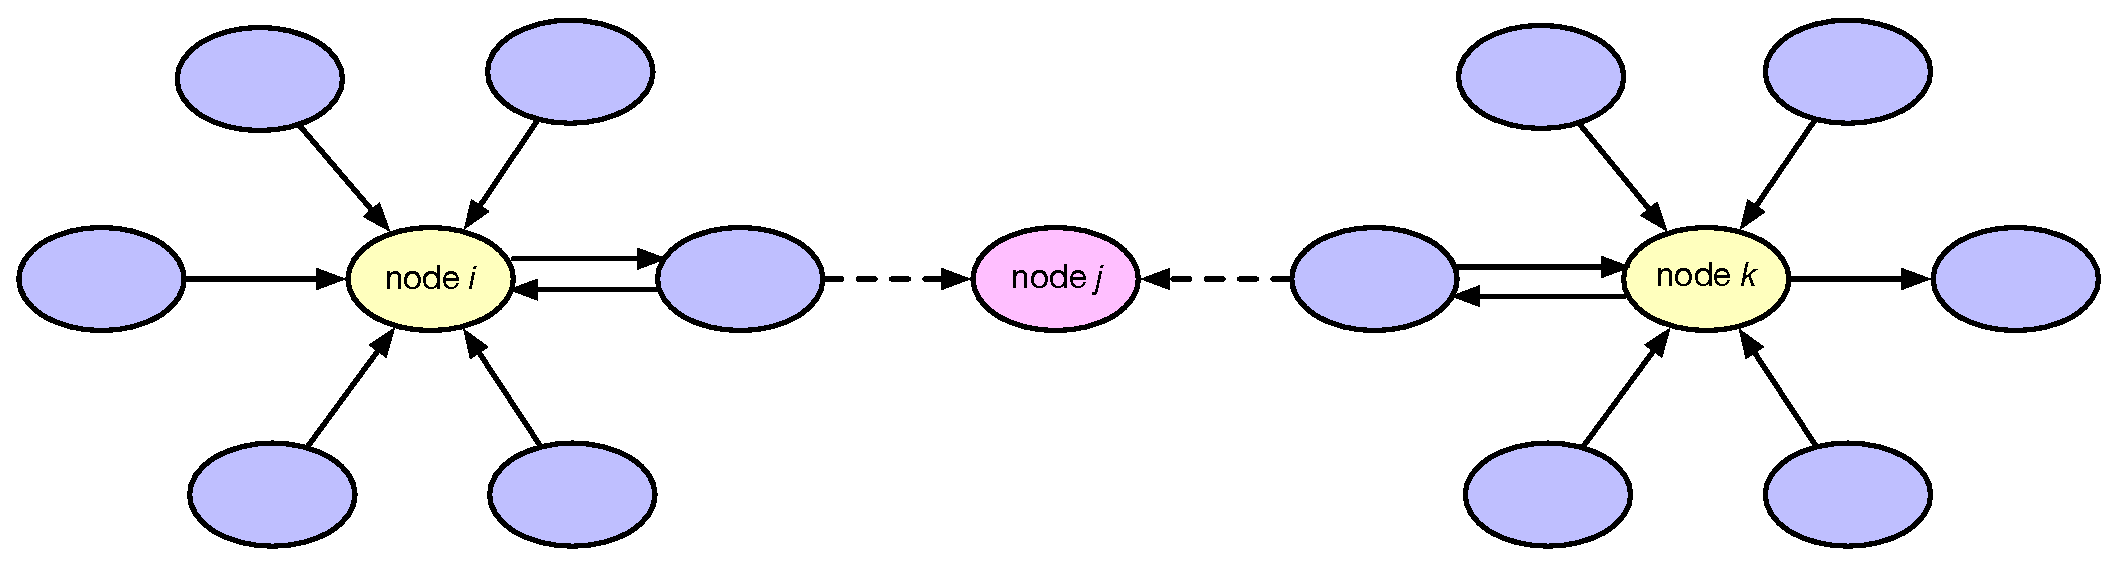
\includegraphics[width=2.0in]{fig/high_order_proximity.eps}
	%\caption{Example of a high-order proximity caption.}
	}
	\subfigure[Example of an asymmetric proximity caption.]{
		\label{fig:asymmetric}
		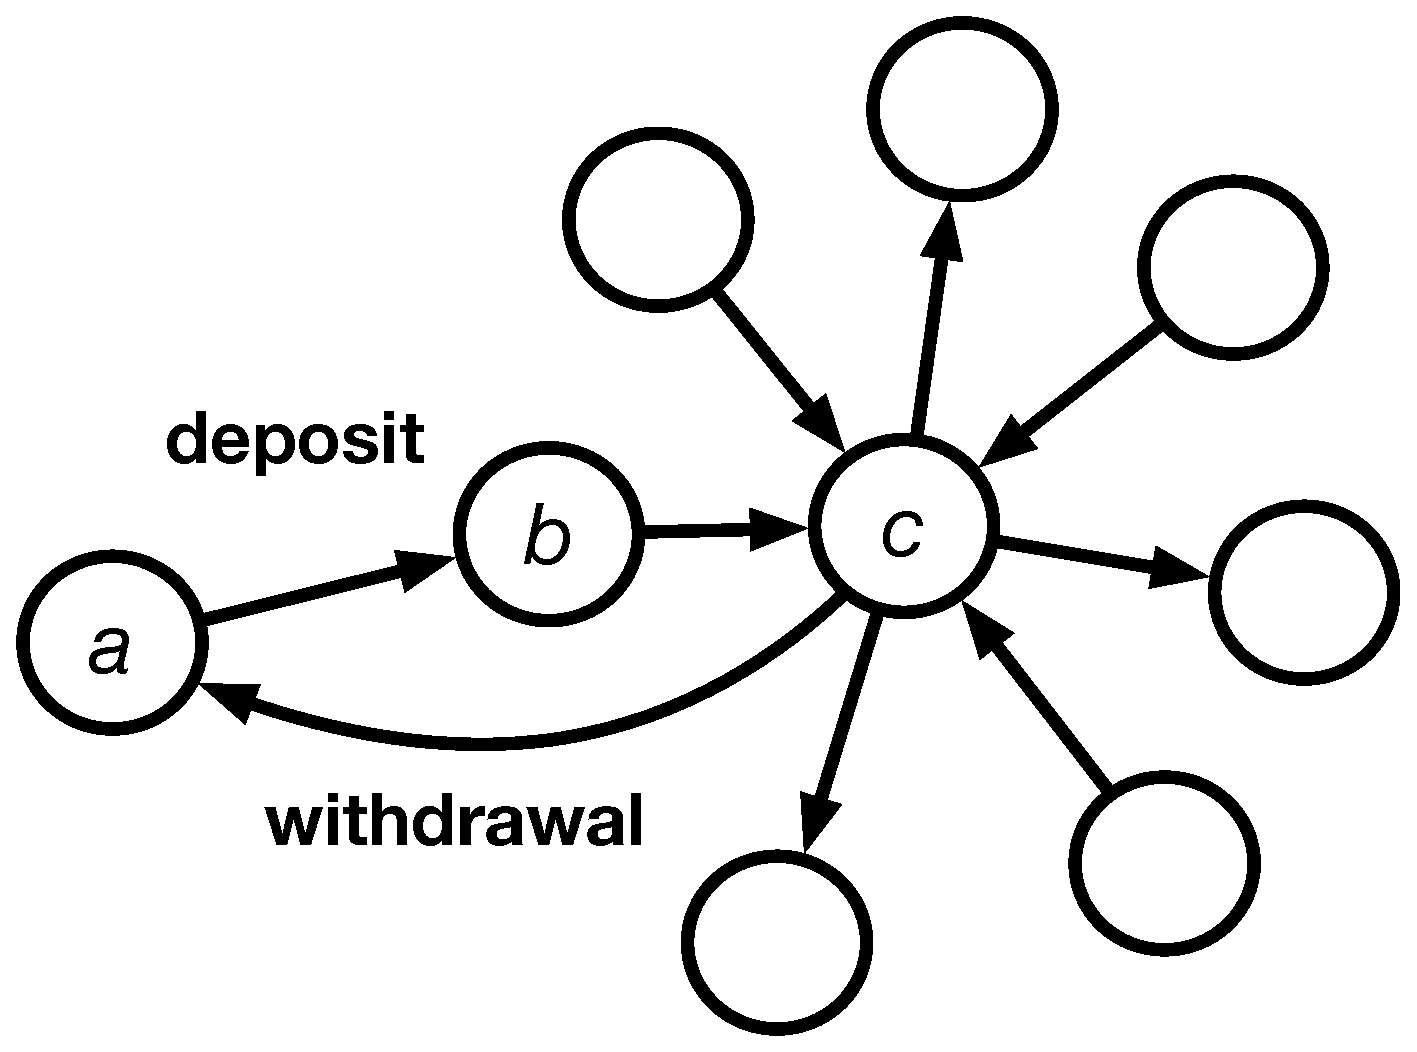
\includegraphics[width=1.5in]{fig/asymmetric.eps}
	}
	\caption{Examples of an asymmetric proximity.}

\end{figure}

To preserve higher order proximities, the hidden layer number in our model is set as 2.

\textcolor{red}{TBA This is second order proximity.}

Another property of closeness in ETG is \emph{asymmetric proximity}. For instance, as shown in Figure. \ref{fig:asymmetric}, node $v_a$ is a Ethereum investor address and node $v_c$ is an exchange root address. Generally, edge weight can be $A_{ab}=A_{bc}=A_{ca}$ since deposit and withdrawal come in pairs in symmetric model. However, the proximity $(v_a,v_c)$is not equal with proximity $(v_c,v_a)$ due to their asymmetric local structures.


 Zhou et. proposed a scalable asymmetric proximity preserving graph embedding method based on random walk~\cite{zhou2017scalable}. In their model, the probability that $v_a$ arrives at $v_c$ is far less than the one that $v_c$ arrives at $v_a$, due to their asymmetric local structures. However, there is no research on asymmetric proximity in GCN model.
 
 To preserve asymmetric proximity, we..
 
 \textcolor{red}{TBA.}

